\chapter{Tinjauan Pustaka}\label{ch:literature}

   \section{Prediksi \textit{Revenue} pada Industri Telekomunikasi}
\label{sec:revenuetelco}

    Layanan SMS internasional merupakan bagian dari ekosistem layanan telekomunikasi lintas negara yang memungkinkan pengiriman pesan singkat antar pengguna di berbagai negara. Layanan ini melibatkan rantai distribusi yang kompleks, mulai dari penyedia layanan di negara asal, \textit{intermediate carrier}, hingga \textit{network operator} di negara tujuan. Kompleksitas rantai distribusi tersebut menyebabkan adanya variasi signifikan pada struktur biaya operasional dan pendapatan yang dihasilkan, terutama pada komponen \textit{international charge} \cite{Truong2021TelecomRevenue}.
    
    Dalam konteks industri telekomunikasi, \textit{revenue} didefinisikan sebagai pendapatan yang diperoleh perusahaan dari penyediaan layanan komunikasi kepada pelanggan. Pada layanan SMS internasional, pendapatan tersebut umumnya direpresentasikan melalui komponen \textit{international 
    charge} yang dibayarkan berdasarkan volume pesan yang dikirimkan lintas negara. Variabel \textit{international charge} sering digunakan sebagai indikator utama \textit{revenue} karena secara langsung mencerminkan nilai transaksi SMS internasional \cite{Truong2021TelecomRevenue}.
    
    Meningkatnya adopsi teknologi alternatif seperti seperti \textit{Flash Calls} yang melewati (\textit{bypass}) jalur SMS tradisional, \textit{gray routes}, serta mode otentikasi alternatif yang lebih murah seperti VOTP \cite{telin2026leakage}. \textit{Flash Calls} merupakan metode otentikasi yang memanfaatkan panggilan telepon singkat yang langsung terputus sebagai pengganti kode OTP berbasis SMS, sehingga trafik SMS A2P untuk keperluan autentikasi beralih ke kanal suara yang tarifnya lebih murah \cite{telin2026leakage}. Kemudian, \textit{Voice OTP} (VOTP) adalah metode pengiriman kode otentikasi melalui panggilan suara otomatis sebagai alternatif SMS yang lebih murah bagi pengirim \cite{telin2026leakage}. Selanjutnya \textit{gray routes} merupakan jalur pengiriman SMS internasional yang memanfaatkan celah jaringan sinyal antara operator untuk meneruskan pesan A2P tanpa melalui kesepakatan interkoneksi resmi sehingga operator tujuan tidak memperoleh pembayaran atas trafik yang masuk. Kondisi ini mendorong perusahaan telekomunikasi untuk mengoptimalkan strategi operasional untuk mempertahankan stabilitas pendapatan.
    
    Pendapatan layanan telekomunikasi, termasuk layanan SMS internasional, dipengaruhi oleh berbagai faktor seperti volume trafik, negara tujuan, jenis layanan, serta karakteristik pelanggan. Hubungan antara faktor-faktor tersebut bersifat non-linear dan dinamis, sehingga 
    menyulitkan penerapan pendekatan statistik konvensional dalam proses prediksi \textit{revenue}. Studi yang dilakukan oleh Danilov dan 
    Maltseva menunjukkan bahwa pendekatan \textit{machine learning} untuk prediksi \textit{revenue} produk telekomunikasi mampu menghasilkan prediksi yang lebih akurat dibandingkan metode konvensional \cite{Danilov2024}. Oleh karena itu, pendekatan berbasis \textit{machine learning} menjadi solusi yang relevan untuk memodelkan pola kompleks dalam data historis trafik SMS internasional \cite{Chen2016}.
    
    Model prediksi \textit{revenue} bertujuan untuk memperkirakan nilai pendapatan di masa depan berdasarkan data historis trafik dan karakteristik layanan. Meskipun beberapa studi telah mengeksplorasi prediksi \textit{revenue} pada layanan telekomunikasi secara umum 
    \cite{Truong2021TelecomRevenue, Danilov2024} serta optimasi 
    hiperparameter berbasis Algoritma Genetika pada model \textit{machine learning} \cite{Ghatasheh2022ModifiedGA}, studi yang secara khusus mengkaji prediksi \textit{revenue} layanan SMS internasional masih sangat terbatas. Prediksi yang akurat dapat digunakan sebagai alat mitigasi risiko finansial dengan mengidentifikasi potensi fluktuasi pendapatan serta mendukung pengambilan keputusan strategis \cite{Oziri2023RevenueForecasting}.

    
    \section{Penelitian Terdahulu}\label{sec:pastresearch}
    Penerapan  algoritma genetika untuk optimasi hiperparameter dilakukan oleh \citeA{gour2024optimizing} dengan menggunakan model \textit{Neural Network} pada dataset diagnosis diabetes. Hasil dari penelitian ini menunjukkan GA konvergen ke nilai hiperparameter yang meningkatkan akurasi. Selain itu, \citeA{Ghatasheh2022ModifiedGA} menerapkan algoritma genetika untuk \textit{hyperparameter optimization} (HPO) pada model XGBoost pada kasus klasifikasi spam dengan \textit{cross-validation} berulang. Penelitian ini menunjukkan hasi G-mean sebesar 82.32 \% dan akurasi 92.67 \% serta mengurangi dimensi fitur kurang dari 10 \%. Selain itu \citeA{Kobayashi2024DQN_BRKGA} melakukan penelitian pendekatan Hybird Deep Q-Network dan Biased Random Key Genetic Algorithm (BRKGA) yang dilakukan pada 8 dateset beragram. \textit{Genetic Algorithm} (GA) terbukti dapat mengurangi biaya komputasi hingga 44 \% tanpa kehilangan kualitas solusi dibanding BRKGA tanpa HPO.
    
    Penerapan GA juga telah diuji secara langsung pada industri telekomunikasi. Misalnya, penelitian oleh \citeA{li2022} mengkombinasikan GA dengan algoritma XGBoost untuk mengoptimalkan parameter model prediksi \textit{churn} pelanggan. Penelitian tersebut menunjukkan bahwa pendekatan GA-XGBoost memberikan hasil yang lebih baik dibandingkan XGBoost tanpa optimasi dengan evaluasi nilai AUC dan F1-Score. Penelitian lain dilakukan oleh \citeA{aljanabi2022distributed} pada kasus \textit{Detection Denial of Service Attacks} (DDoS) pada \textit{Software Define Networks} (SFD). Studi tersebut menunjukkan GA mengoptimalkan hiperparameter model \textit{Decision Tree} sehingga mencapai akurasi 99.49 \% pada kasus klasifikasi \textit{traffic}. Berdasarkan berbagai penelitian terdahulu tersebut, dapat disimpulkan bahwa metode optimasi berbasis GA telah terbukti efektif untuk meningkatkan kinerja model \textit{machine learning} di berbagai domain, termasuk telekomunikasi. Namun, sebagian besar penelitian belum ditemukan aplikasi GA untuk optimasi hiperparameter \textit{tree-based models} untuk prediksi pendapatan layanan komunikasi internasional. Dengan demikian, untuk menjawab permasalahan tersebut penelitian ini menerapkan GA sebagai metode optimasi hiperparameter pada \textit{tree-based models} untuk memprediksi prediksi layanan komunikasi internasional. Pendekatan ini diharapkan dapat memberikan kontribusi baik dalam mengurangi \textit{error} atau kesalahan prediksi pendapatan di industri telekomunikasi serta mengevaluasi dampak optimasi terhadap akurasi prediksi dan efisiensi komputasi.

    \section {Konsep Dasar Klasifikasi}
    Klasifikasi merupakan metode \textit{machine learning} dalam data mining untuk memprediksi anggota dari tiap grup data. Meskipun banyak metode yang ada pada \textit{machine learning}, klasifikasi merupakan metode yang paling banyak digunakan \cite{inproceedings}. Klasifikasi merupakan metode yang paling banyak dipelajari dan diteliti oleh para \textit{researcher} di bidang data mining dan machine learning. Output pada klasifikasi berupa variable yang memiliki label kelas. Metode klasifikasi sendiri dibedakan menjadi dua yaitu \textit{binary classification} dan \textit{multiclass classification}. \textit{Binary classification} merupakan metode klasifikasi yang memprediksi dua kelas yaitu antara 0 dan 1. Sedangkan \textit{multiclass classification} merupakan metode yang memprediksi lebih dari dua kelas \cite{ng2023cs229}. Pada penelitian Tugas Akhir ini digunakan metode \textit{binary classification} karena tujuan klasifikasi untuk memprediksi transaksi yang mempunyai pendapatan nol (tidak aktif) dan transaksi yang mempunyai pendapatan tidak nol (aktif).
    
    \section {Konsep Dasar Regresi}
    Regresi merupakan metode statistika yang digunakan untuk memodelkan hubungan antara variabel dependen atau target dengan satu atau lebih variabel independen atau prediktor. Regresi memiliki tujuan utama untuk memahami bagaimana nilai variabel dependen berubah ketika salah satu variabel independen diubah, sementara variabel independen lainnya tetap konstan. Menurut James et al. (2023), regresi telah menjadi salah satu metode fundamental dalam statistika dan \textit{machine learning} yang digunakan secara luas dalam berbagai domain aplikasi, mulai dari ekonomi, bisnis, hingga ilmu sosial.
    
    \begin{equation} \label{eq:wmape}
        Y = f(x) + \varepsilon
    \end{equation}
     
   Secara matematis, model regresi dapat dinyatakan pada persamaan 2.1 di mana $Y$ adalah variabel dependen yang ingin diprediksi, $X$ adalah vektor variabel independen yang terdiri dari $X_1, X_2, \dots, X_p$, $f(X)$ adalah fungsi sistematis yang menggambarkan hubungan antara $X$ dan $Y$, dan $\varepsilon$ adalah komponen \textit{error} atau \textit{noise} acak yang merepresentasikan variabilitas dalam data yang tidak dapat dijelaskan oleh model. Pemodelan regresi berusaha untuk menemukan fungsi $f(X)$ yang paling baik merepresentasikan hubungan tersebut berdasarkan data observasi yang ingin diprediksi \cite{hastie2009elements}.
    
    Pemilihan model regresi yang tepat dan konfigurasi hiperparameter sangat mempengaruhi performa. Misalnya parameter seperti jumlah pohon (\textit{estimators}), kedalaman maksimum (\textit{max depth}), tingkat pembelajaran (\textit{learning rate}), atau ukuran sampel bawah (\textit{min samples leaf}) dapat berdampak besar terhadap keseimbangan bias dan \textit{varians}. Untuk itu, metode optimasi seperti GA ditempatkan sebagai layer pencarian hiperparameter di atas model regresi ini. 

    \section{Two Staged Models}
    \textit{Two-stage models} atau model dua tahap merupakan pendekatan pemodelan 
    prediktif yang membagi proses prediksi menjadi dua fase yang saling berurutan. Model awal menghasilkan informasi atau keluaran tertentu kemudian keluaran dari tahap 
    pertama tersebut digunakan sebagai masukan tambahan untuk model pada tahap 
    kedua \cite{en10101547}.
    
    Secara umum, struktur \textit{two-stage models} dapat direpresentasikan sebagai 
    berikut. Misalkan $\mathbf{x} \in \mathbb{R}^p$ adalah vektor fitur masukan, 
    maka tahap pertama menghasilkan keluaran $z = f_1(\mathbf{x})$ dan tahap kedua 
    menghasilkan prediksi akhir $\hat{y} = f_2(\mathbf{x}, z)$. Maka dari itu, 
    prediksi akhir secara keseluruhan dapat dituliskan pada persamaan 2.2.
    
    \begin{equation}
        \hat{y} = f_2\!\left(\mathbf{x},\; f_1(\mathbf{x})\right)
    \end{equation}
    
    Keunggulan utama pendekatan ini dibandingkan model satu tahap adalah kemampuannya 
    untuk memecah masalah yang kompleks menjadi dua sub-masalah yang lebih 
    sederhana dan lebih mudah dioptimalkan secara terpisah \cite{en10101547}. 
    Output dari model tahap pertama menjadi informasi yang berharga bagi model tahap kedua, sehingga model tahap kedua dapat menangkap pola data yang tidak dapat ditangkap jika hanya menggunakan fitur data tanpa melalui tahap model pertama. 
    
    \section{Tree-based Models}
    
    Model berbasis pohon (\textit{tree-based models}) merupakan salah satu pendekatan pembelajaran mesin yang sering digunakan karena kemampuannya dalam memodelkan hubungan non-linier serta hubungan kompleks antar fitur tanpa memerlukan asumsi distribusi data tertentu. Model ini bekerja dengan membagi ruang fitur ke dalam beberapa region menggunakan aturan pemisahan berbasis kriteria tertentu, seperti \textit{Gini impurity} atau \textit{information gain}, sehingga menghasilkan struktur hierarkis berbentuk pohon keputusan.
    
    \textit{Decision Tree} merupakan bentuk paling dasar dari model berbasis pohon. Model ini melakukan pemisahan data secara rekursif berdasarkan fitur yang paling informatif hingga mencapai kondisi berhenti tertentu. Meskipun mudah diinterpretasikan dan efisien secara komputasi, \textit{Decision Tree} memiliki kelemahan utama berupa kecenderungan terhadap \textit{overfitting}, terutama ketika pohon tumbuh terlalu dalam \cite{info14030140}.

    % \begin{figure}[H]
    % \centering
    %     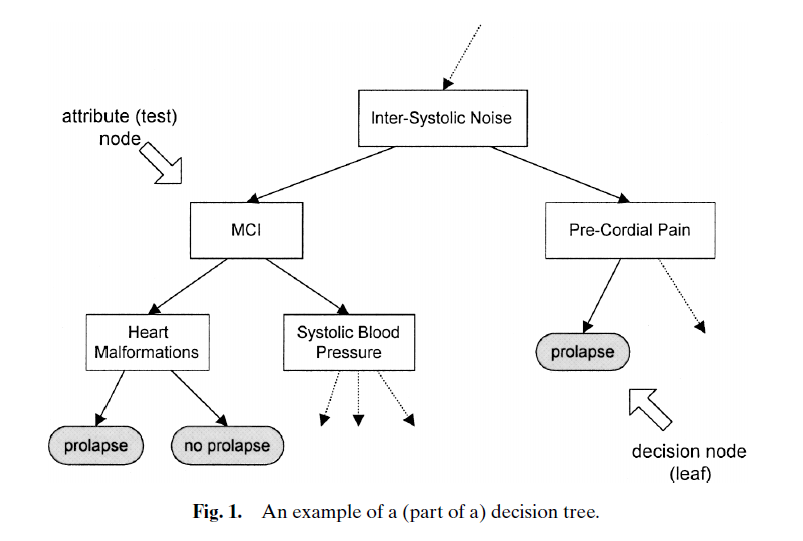
\includegraphics[width=0.8\textwidth]{tugas-akhir/assets/images/dt.png}
    %     \caption {Model \textit{Decision Tree} dalam dunia medis}
    %     \text{\cite{Wang2023RUL}}
    %     \label{fig:revenue-framework}
    % \end{figure}

    
    \subsection{Random Forest}
    \textit{Random Forest} merupakan kombinasi \textit{multiple decision trees} untuk meningkatkan akurasi prediksi dan mengurangi \textit{overfitting} \cite{Breiman2001}. Algoritma \textit{Random Forest} berjalan dengan membentuk sekumpulan pohon keputusan yang dilatih menggunakan sample acak dari data latih dengan pengembalian (\textit{boostrap sampling}), serta memilih subset fitur secara acak pada setiap \textit{leaf} pohon. Proses ini menghasilkan variasi antar pohon yang  mengurangi korelasi internal, sehingga meningkatkan kemampuan generalisasi model. Hasil dari tiap pohon digabungkan dengan menggunakan \textit{vote majority} dalam menghaasilkan hasil klasifikasi atau rata-rata prediksi untuk regresi yang lebih stabil dan akurat \cite{MontesinosLópez2022}. Prediksi akhir dari \textit{Random Forest} untuk masalah regresi dihitung sebagai rata-rata dari prediksi seluruh \textit{trees} dalam \textit{ensemble} yang dapat dilihat pada persamaan 2.2.
    \begin{equation}
        \hat{y} = \frac{1}{B} \sum_{b=1}^{B} f_b(x)
    \end{equation}
    di mana $B$ adalah jumlah \textit{tree} dalam \textit{ensemble} dan $f_b(x)$ adalah prediksi dari \textit{tree} ke-$b$ untuk input $x$. Kelebihan \textit{Random Forest} adalah kemampuan menangani \textit{overfitting} dengan baik, \textit{robust} terhadap \textit{outlier}, dan dapat memberikan estimasi \textit{feature importance} yang berguna untuk interpretasi model.

    % \begin{figure}[H]
    % \centering
    %     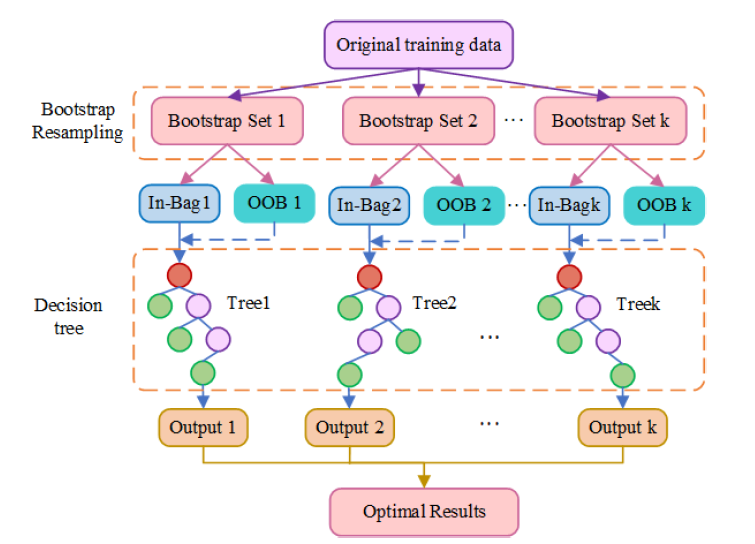
\includegraphics[width=0.8\textwidth]{tugas-akhir/assets/images/RandomForest.png}
    %     \caption {Struktur \textit{Random Forest}}
    %     \text{\cite{Wang2023RUL}}
    %     \label{fig:revenue-framework}
    % \end{figure}
    
    
    \subsection{XGBoost (Extreme Gradient Boosting)}
    XGBoost merupakan kombinasi \textit{decision tree } yang mengimplementasikan \textit{gradient boosting} yang sangat teroptimasi. XGBoost pertama kali dikembangkan oleh Chen Tianqi dan Carlos pada tahun 2016 dan dilanjutkan oleh peneliti selanjutnya untuk melakukan penyempurnaan dari penelitian sebelumnya \cite{10.1371/journal.pone.0283452}. 
    
    
    XGBoost merupakan model yang menggunakan pendekatan \textit{boosting}, yaitu membangun model secara bertahap di mana setiap model baru berusaha belajar dari kesalahan yang dibuat dari model sebelumnya. Berbeda dengan metode \textit{bagging}, seperti \textit{Random Forest},\textit{ boosting} bersifat sekuensial dan lebih fokus pada observasi yang susah diprediksi oleh model sebelumnya \cite{Dong2020}. Kelebihan XGBoost adalah penggunaan \textit{regularized objective function} yang membantu mengurangi \textit{overfitting} dan meningkatkan generalisasi model. Formula dari XGBoost dapat dilihat pada persamaaan 2.3.
    \begin{equation}
    \hat{y}_i^{(m)} = \sum_{k=1}^{m} f_k(x_i), \quad f_k \in F
    \tag{2.7}
    \end{equation}
    
    di mana $\hat{y}_i^{(m)}$ adalah prediksi pada iterasi ke-$m$ dengan $m$ adalah indeks
    dari jumlah iterasi, $f_k$ adalah fungsi pohon keputusan ke-$k$, dan $F$ adalah
    ruang fungsi semua pohon yang mungkin. Pelatihan XGBoost bertujuan untuk
    meminimalkan fungsi objektif pada persamaan (2.8):
    
    \begin{equation}
    \mathcal{L}^{(m)} = \sum_{i=1}^{n} l(y_i, \hat{y}_i^{(m)}) + \sum_{k=1}^{m} \Omega(f_k)
    \tag{2.8}
    \end{equation}
    
    di mana $\mathcal{L}^{(m)}$ adalah fungsi objektif yang diminimalkan pada iterasi
    \textit{boosting} ke-$m$, $l$ adalah fungsi \textit{loss} yang mengukur selisih antara
    nilai aktual dan prediksi, $\hat{y}_i$ adalah nilai prediksi model, dan $\Omega$
    adalah fungsi regularisasi seluruh pohon keputusan. fungsi regularisasi pada XGBoost dapat dituliskan lebih lanjut pada
    persamaan (2.9):
    
    \begin{equation}
    \Omega(f) = \gamma T + \frac{1}{2}\lambda \|w\|^2
    \tag{2.9}
    \end{equation}
    
    di mana $\gamma$ adalah parameter regularisasi struktural
    (\textit{tree complexity penalty}) yang berfungsi untuk mengontrol penalti terhadap jumlah daun,
    $T$ sebagai jumlah daun, dan $w$ sebagai bobot prediksi pada setiap \textit{leaf node}
    (\textit{leaf weight}) dalam pohon keputusan XGBoost \cite{Chen2016}.
    
    % \begin{figure}[H]
    % \centering
    %     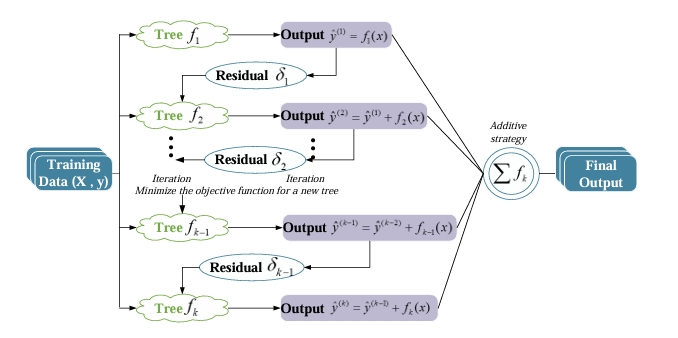
\includegraphics[width=0.8\textwidth]{tugas-akhir/assets/images/XGBoost.png}
    %     \caption {Struktur \textit{XGBoost}}\text{\cite{Cheng2020SPSEXGBoost}}\label{fig:revenue-framework}
    % \end{figure}
    
    % \subsection{LightGBM (Light Gradient Boosting Machine)}
    % LightGBM dikembangkan oleh Microsoft Research dengan fitur utama \textit{Gradient-based One-Side Sampling} (GOSS) dan \textit{Exclusive Feature Bundling} (EFB) yang membuatnya sangat efisien untuk dataset berdimensi tinggi \cite{Ke2017}. Perbedaan dasar LightGBM adalah penggunaan strategi \textit{leaf-wise tree growth} yang diformulasikan pada persamaan 2.5.
    % \begin{equation}
    %     \Delta\text{loss} = \max\{\Delta\text{loss}(\text{leaf}_i)\}
    % \end{equation}
    % Strategi ini memilih \textit{leaf} dengan pengurangan \textit{loss} maksimum untuk di-\textit{split} selanjutnya. Berbeda dengan strategi \textit{level-wise} yang digunakan oleh sebagian besar implementasi GBDT, pendekatan \textit{leaf-wise} ini dapat mempercepat proses training hingga 20 kali lipat sambil mempertahankan akurasi yang sebanding \cite{Ke2017}.
    
    % \subsection{CatBoost (Categorical Boosting)}
    % CatBoost, dikembangkan oleh Yandex, menggunakan teknik \textit{ordered boosting} dan penanganan fitur kategorikal khusus untuk mengatasi \textit{prediction shift} yang disebabkan oleh \textit{target leakage}. Prediksi untuk sampel $i$ diformulasikan pada persamaan 2.6.
    % \begin{equation}
    %     \hat{y}_i = \sum_{t=1}^{T} \alpha_t \times \text{tree}_t(x_i; M_t^i)
    % \end{equation}
    % Untuk menangani fitur kategorikal, CatBoost menggunakan statistik target dengan formula pada persamaan 2.7.
    % \begin{equation}
    %     TS_k = \frac{\sum_{i:x_{i,k}=c} y_i + a p}{\sum_{i:x_{i,k}=c} 1 + a}
    % \end{equation}
    % di mana $a$ adalah parameter \textit{smoothing} dan $p$ adalah nilai prior. Teknik \textit{ordered boosting} yang diimplementasikan CatBoost secara efektif mengurangi \textit{overfitting} dibandingkan dengan metode boosting tradisional \cite{Prokhorenkova2018}.
        
    \section{Metode Optimasi hiperparameter}

    Dalam proses pelatihan model machine learning seperti proses optimasi hiperparameter  masih dibutuhkan. Banyak algoritma yang memiliki banyak hyperparamater sehingga proses optimasi hiperparameters menjadi lebih kompleks. Metode yang tidak terlalu kompleks adalah \textit{manual tuning} atau pencarian parameter secara manual. Akan tetapi, metode ini sangat bergantung kepada seberapa kompleks masalah yang ingin diselesaikan. Karena banyaknya kemungkinan yang dapat dihasilkan, solusi yang dihasilkan butuh untuk diskalasikan. Beberapa metode terkenal yang sering digunakan adalah \textit{grid search}, \textit{random search}, \textit{bayesian optimization}, serta pendekatan secara heuristik seperti Algoritma Genetika \cite{10.1145/3297067.3297080}.

    Masalah utama dalam optimasi hiperparameter model \textit{machine learning} adalah efisiensi waktu dan ruang pencarian. Optimasi Bayesian meningkatkan efisiensi waktu metode pencarian grid, tetapi metode ini bekerja dengan ruang pencarian yang terbatas seperti metode pencarian grid begitupun dengan random search. Di sisi lain, GA telah mengatasi kedua masalah tersebut, yaitu dengan mencari di berbagai ruang yang lebih luas dengan waktu yang lebih efisien \cite{Katoch2021}. Maka dari itu, GA membantu model \textit{TreeBased Models} seperti XGBoost memiliki performa yang lebih baik. GA membantu mengevaluasi berbagai solusi yang lebih luas dengan cepat untuk menemukan pilihan terbaik. Hai ini sangat penting untuk merancang sistem pendukung keputusan klinis (\textit{Decision Support System}) dan analisis big data \cite{https://doi.org/10.1155/2023/9673395}.
    
    % \subsection{Optimasi \textit{Grid Search}}
    % Strategi yang dikenal sebagai grid search mengotomatisasi metode \textit{trial-and-error} dengan menyediakan daftar nilai parameter yang mungkin untuk dipilih. Strategi ini terkenal penggunaannya dalam machine learning untuk mengidentifikasi pengaturan parameter yang optimal bagi model seperti yang ditunjukkan pada gambar 2.5.

    % \begin{figure}[H]
    % \centering
    %     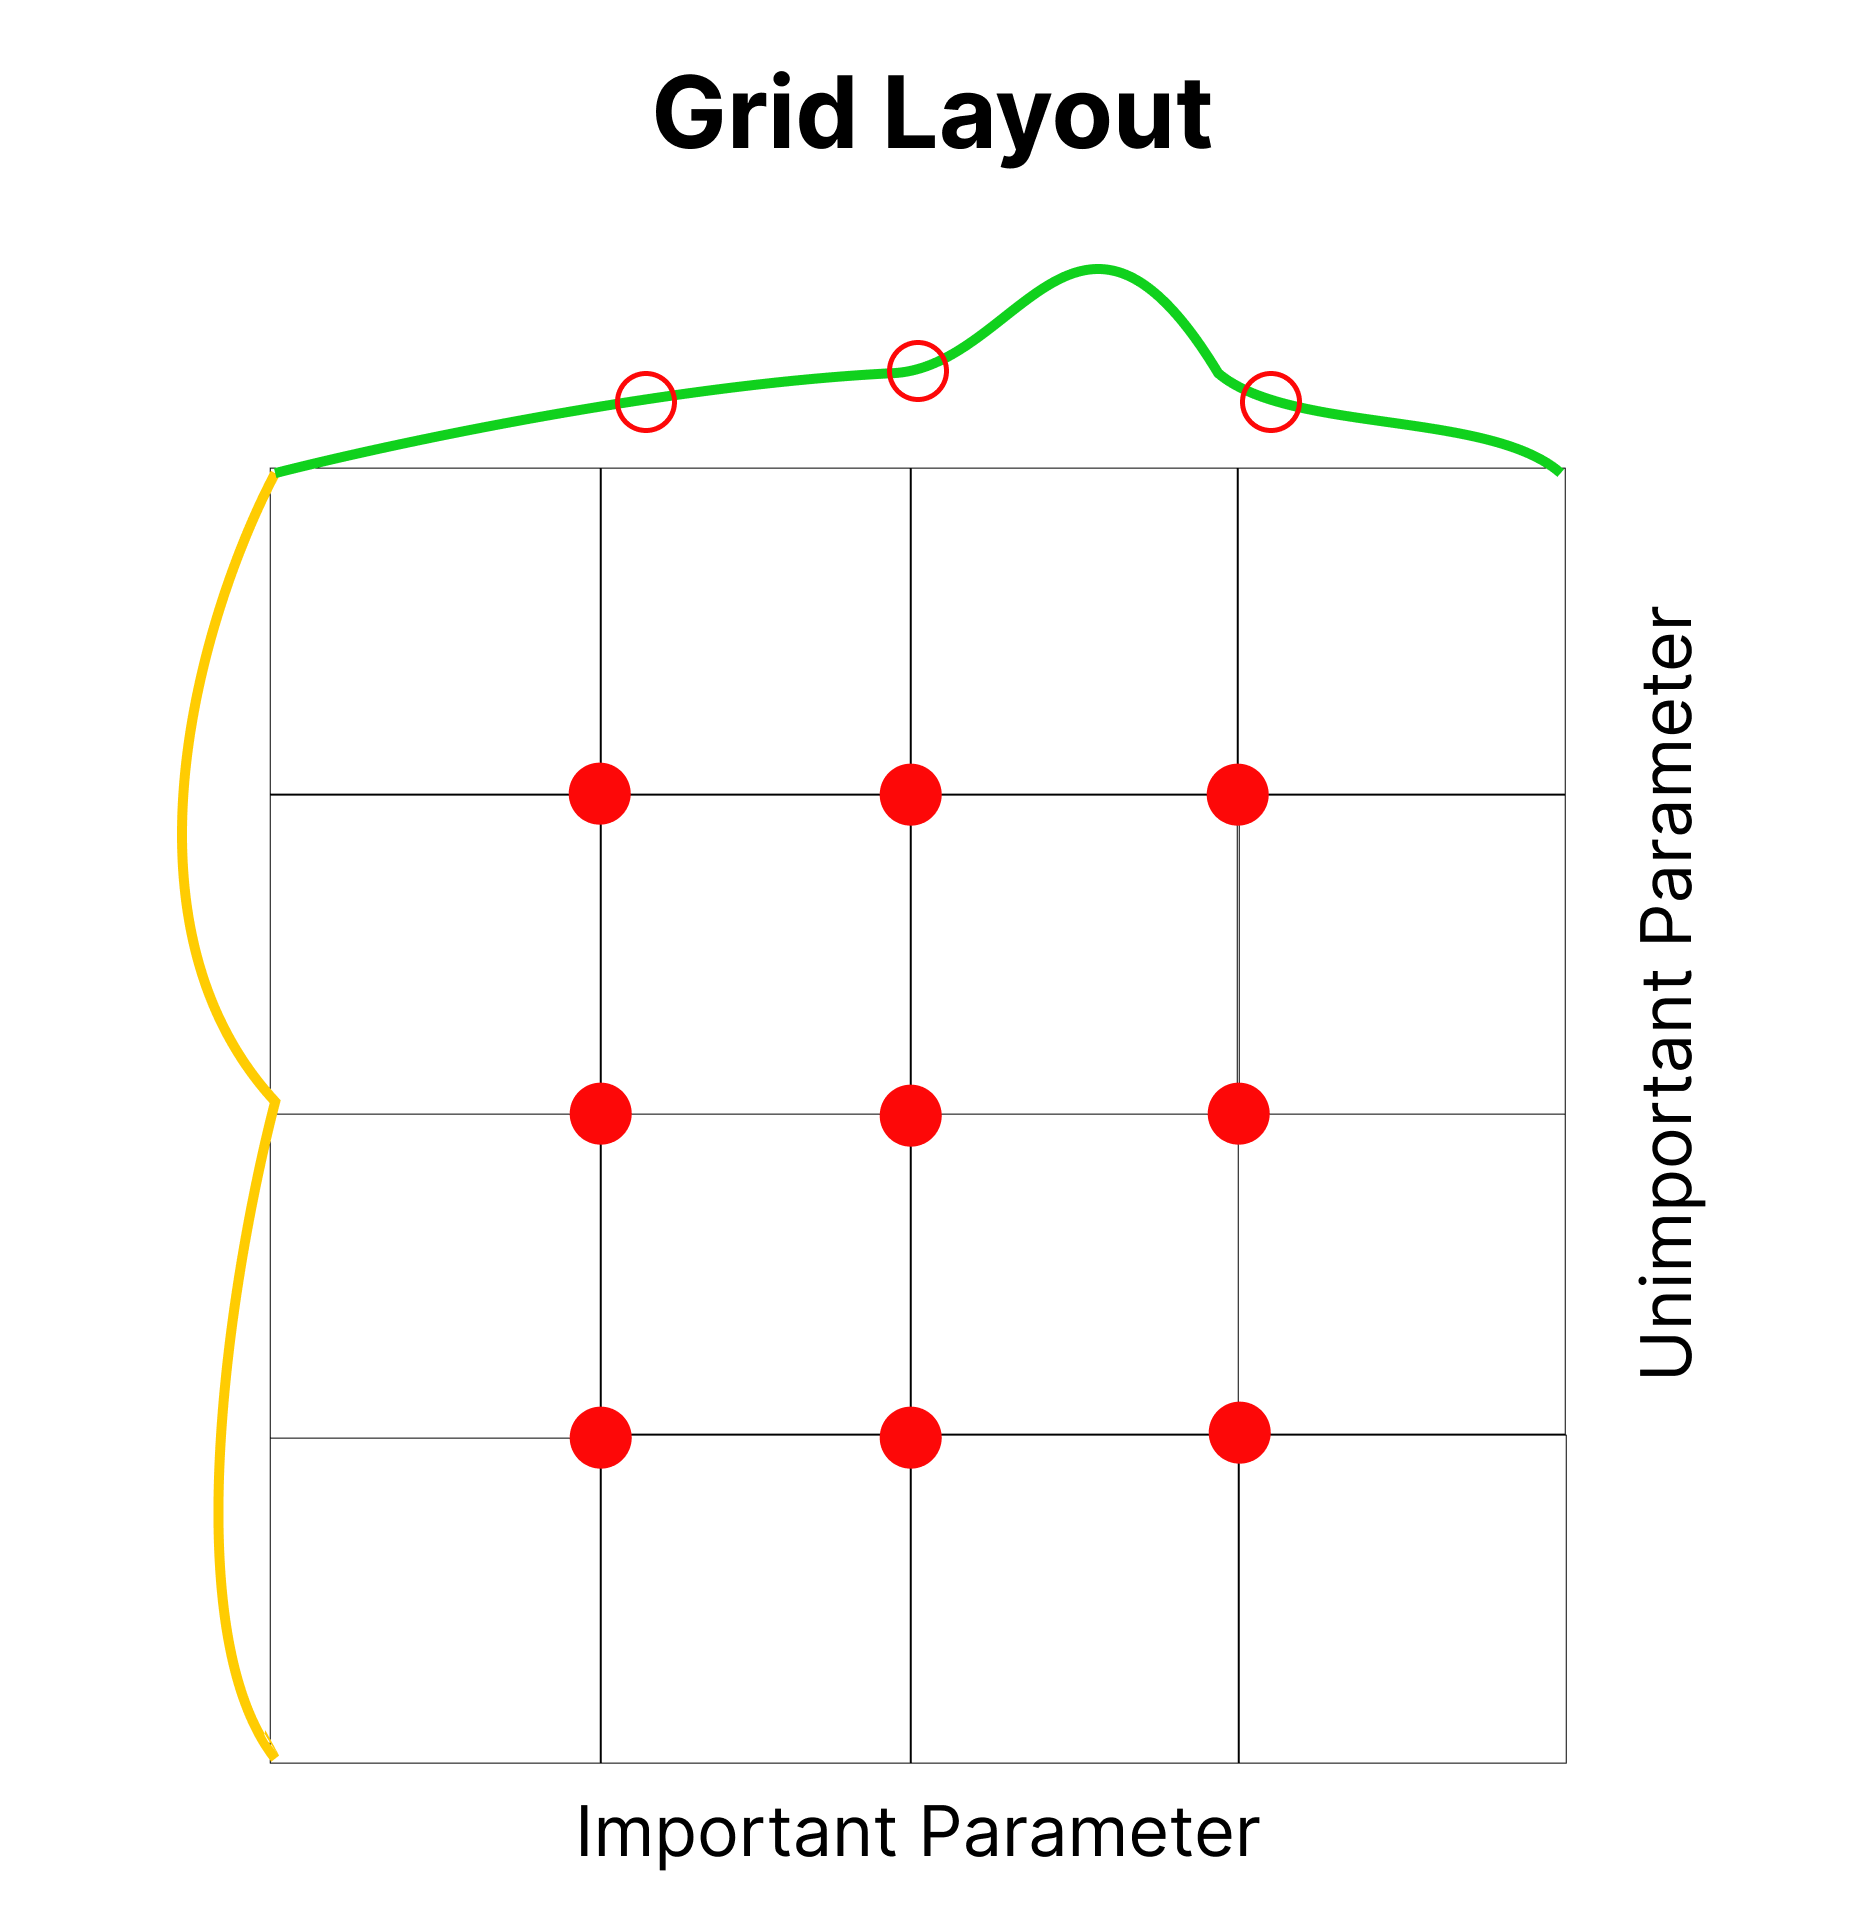
\includegraphics[width=0.5\textwidth]{tugas-akhir/assets/images/Grid Search.png}
    %     \caption {Metode \textit{Grid Search}}
    %     \text{\cite{Shanthi2023}}
    %     \label{fig:revenue-framework}
    % \end{figure}
    
    % Ketika mencoba memilih model terbaik untuk semua kemungkinan pengaturan hiperparameter, dimulai dengan membangun model untuk setiap kemungkinan konfigurasi nilai hiperparameter, kemudian mengevaluasi setiap model dan memilih satu yang berkinerja terbaik. Untuk membangun \textit{grid variabel hiperparameter}, nilai grid dibuat terpisah untuk setiap kombinasi hiperparameter dan kemudian melatih model pada data validasi untuk setiap nilai grid.
    
    % Strategi ini mencoba mencari setiap konfigurasi hiperparameter yang mungkin, yang membuat metode ini menjadi pendekatan yang tidak efisien. Kelemahan lain dari \textit{grid search} adalah metode ini mungkin mengalami masalah dimensi ketika jumlah hiperparameter tumbuh secara eksponensial. Namun, tidak ada jaminan bahwa pencarian ini akan selalu memberikan jawaban yang sempurna

    % \subsection{Optimasi \textit{Random Search}}
    % Metode \textit{random search} bekerja dengan mengambil sampel nilai secara  acak untuk memperkirakan fungsi objektif. Metode ini efisien karena tidak mengasumsikan apa pun tentang struktur fungsi target. Metode ini sangat berguna ketika terdapat sejumlah besar pengetahuan domain yang harus dihadapi, yang memungkinkan munculnya solusi yang berlawanan dengan intuisi. Dibandingkan dengan \textit{grid search}, random search jauh lebih efektif dalam mengidentifikasi nilai terbaik seperti yang ditunjukkan pada gambar 2.6.

    % \begin{figure}[H]
    % \centering
    %     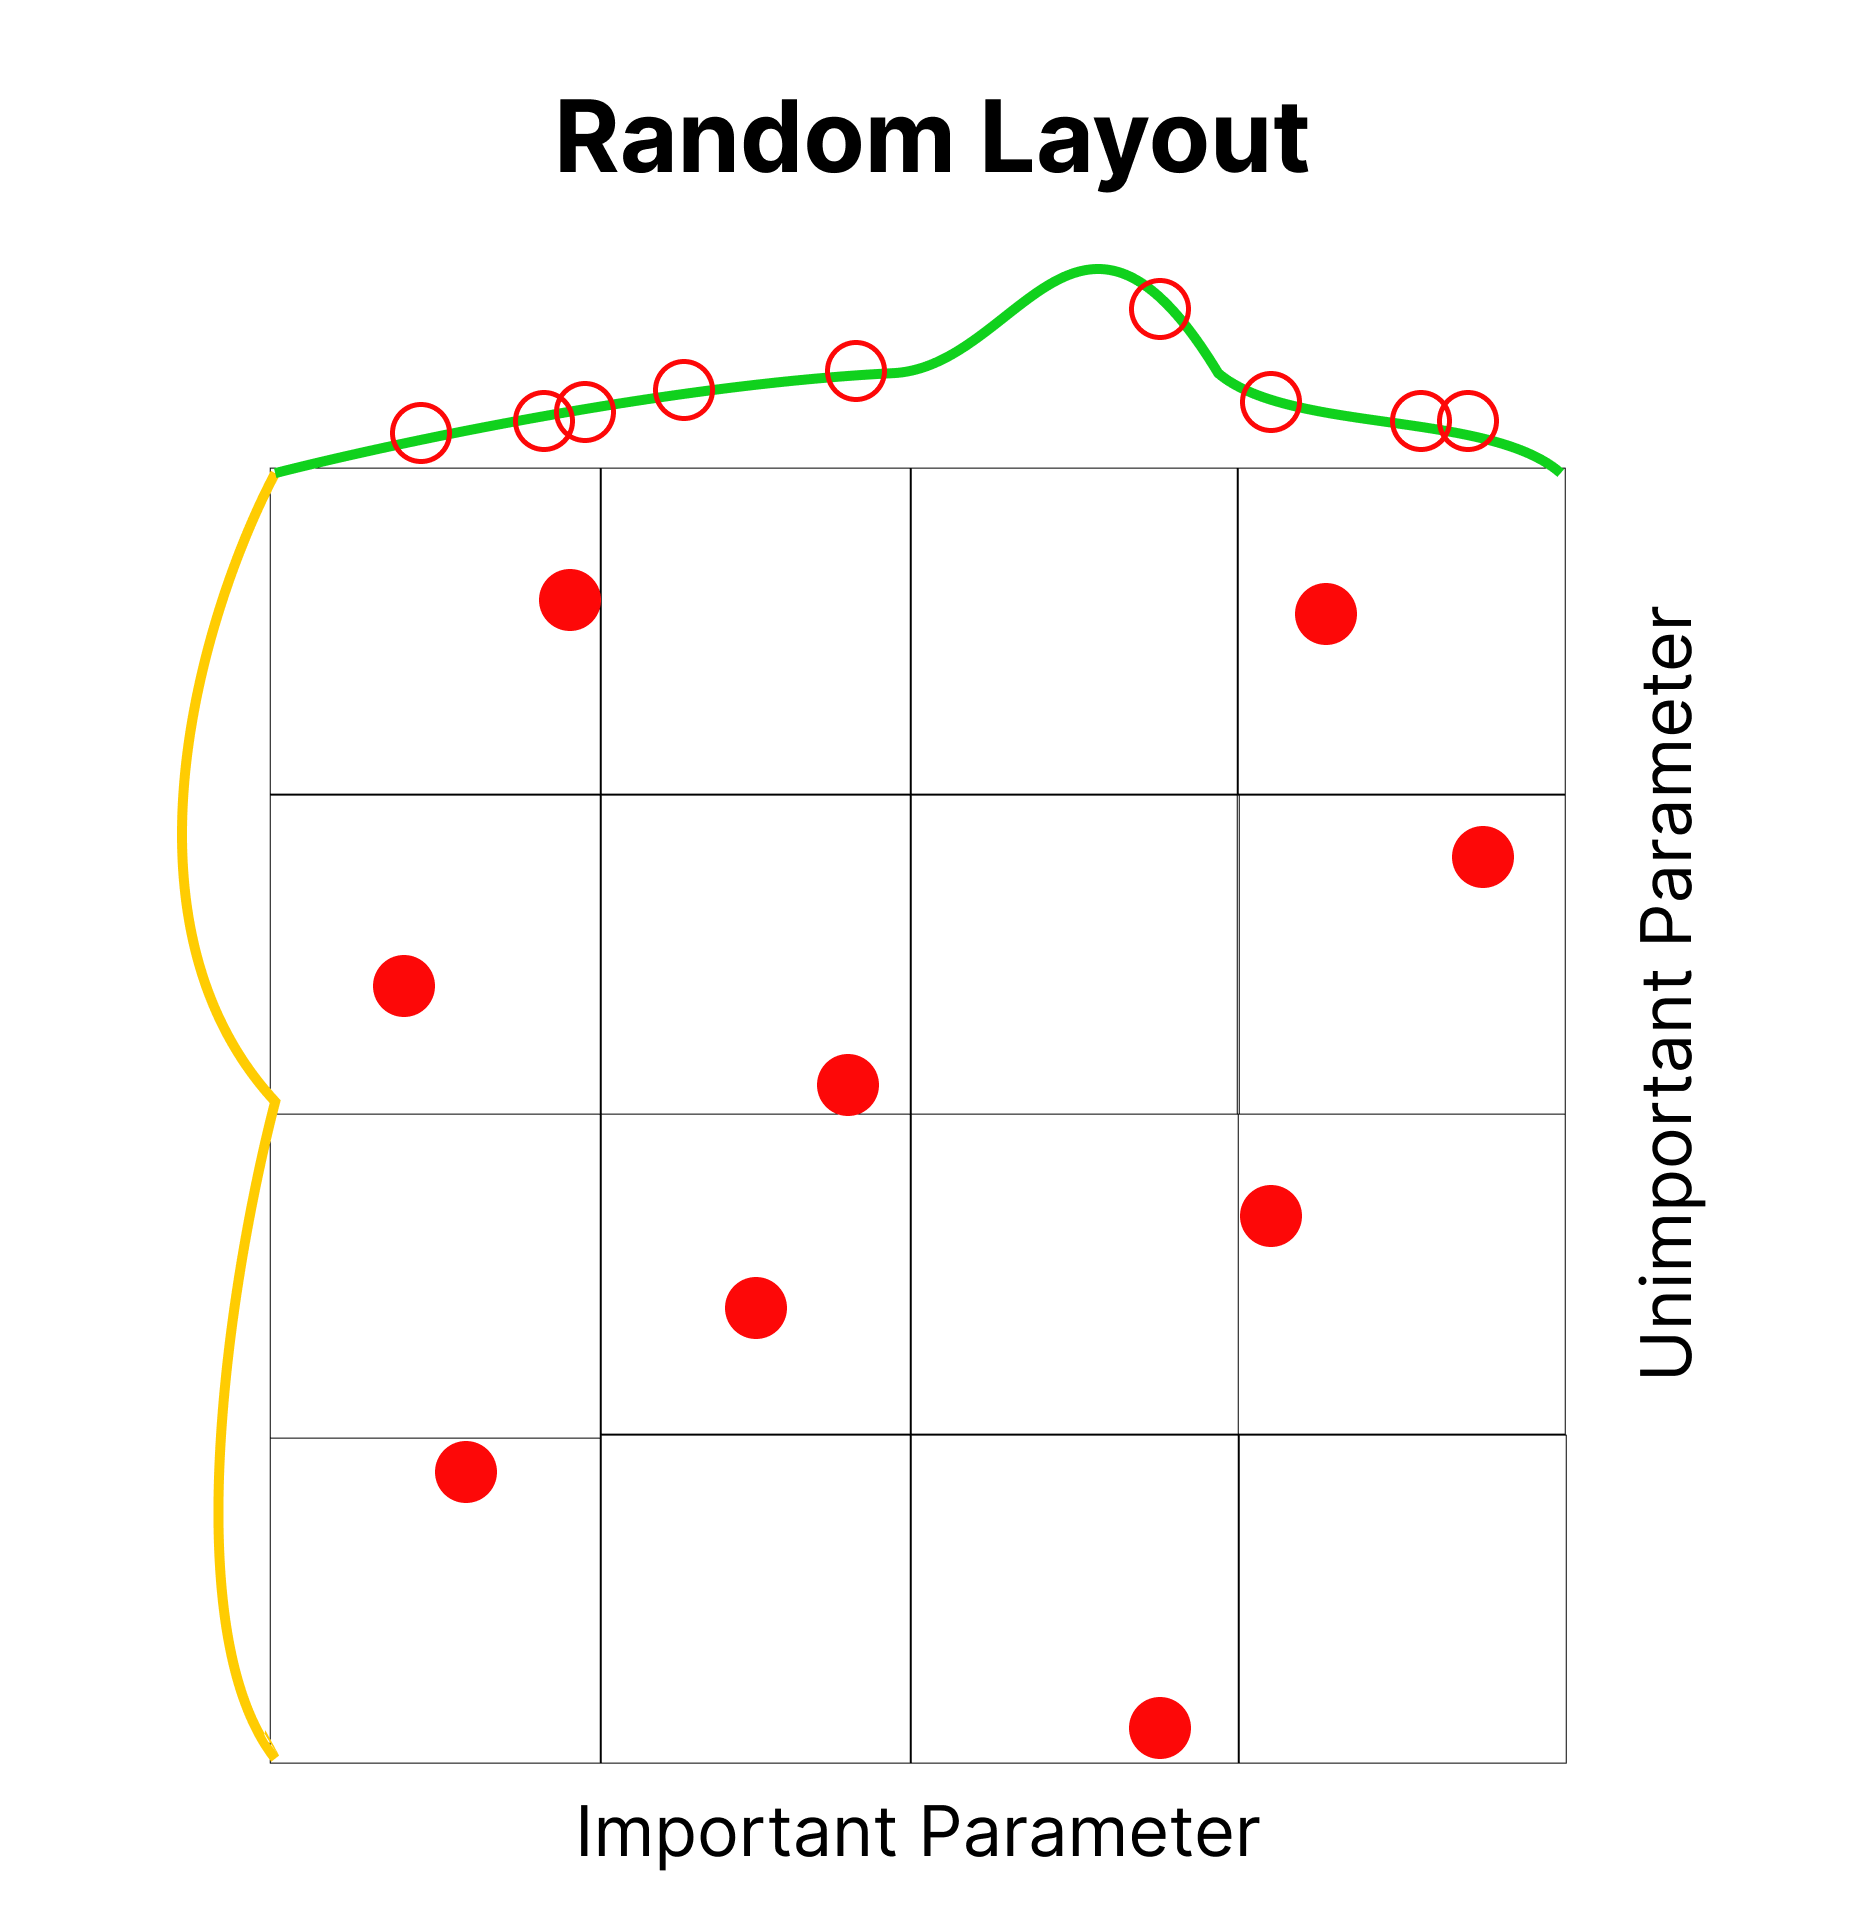
\includegraphics[width=0.5\textwidth]{tugas-akhir/assets/images/Random Search.png}
    %     \caption {Metode \textit{Random Search}}
    %     \text{\cite{Shanthi2023}}
    %     \label{fig:revenue-framework}
    % \end{figure}
    
    % Langkah-langkah dari metode ini meliputi penentuan ruang lingkup hiperparameter kemudian pemilihan kombinasi secara acak untuk melatih dan menguji model. Akan tetapi, ketika hanya sedikit hiperparameter yang memengaruhi kinerja algoritma machine learning, \textit{grid search} dapat mengungguli metode \textit{random search}. 
    
    % Ketika mencari sesuatu yang kompleks, seperti data yang bising (noisy) atau terputus-putus, random search sangat efisien dan menggunakan memori minimal. Karena itu, sampel input yang besar mungkin menjadi pilihan yang lebih baik. Setiap sampel bersifat unik, yang berarti jika sampel harus dianalisis secara paralel untuk mempercepat proses,  penemuan parameter optimal tetap efektif tanpa mengurangi keandalan hasil temuan.\cite{Shanthi2023}.

    \subsection{Algortima Genetika}\label{sec:ga}
    
    Algoritma Genetika (Genetic Algorithm) merupakan salah satu algoritma optimasi metaheuristik berbasis populasi yang terinspirasi dari teori seleksi alam. Populasi baru dihasilkan dengan berulang kali menggunakan operator genetik pada setiap individu dalam populasi. Istilah-istilah penting dari algoritma ini adalah pembentukan kromosom, inisialisasi populasi, seleksi (selection), \textit{crossover}, mutasi, dan fungsi \textit{fitness}. \shortciteA{Katoch2021} menjelaskan bahwa proses \textit{Genetic Algorithm} (GA) dimulai dengan pembentukan pulasi awal Y yang terdiri dari n kromosom secara acak, di mana n adalah ukuran populasi yang ditentukan sebelumnya. Setiap kromosom merepresentasikan satu kandidat solusi yang terdiri dari sejumlah gen sebanyak hiperparameter yang ingin dioptimasi. Dua kromosom yaitu C1 dan C2, dipilih dari populasi berdasarkan nilai \textit{fitnessnya}. C1 dan C2 akan menghasilkan keturunan baru O dengan melalui proses \textit{crossover}. Probabilitas pada tahap ini dinamakan $P_c$, yang merupakan parameter probabilitas \textit{crossover}. Operator mutasi genetik dengan probabilitas $P_m$ kemudian diterapkan pada O untuk menghasilkan anggota baru O’. Anggota O’ ditambahkan ke populasi sebelumnya untuk membentuk populasi baru. Proses seleksi, crossover, dan mutasi berlanjut hingga seluruh populasi dengan nilai \textit{fungsi fitness} yang optimal dihasilkan. Probabilitas crossover dan mutasi inilah yang menyebabkan GA dapat secara dinamis mencari solusi optimal.


    \section{Penerapan Algoitma Genetika untuk Optimasi hiperparameter \textit{Tree-Based Models}}

    Penerapan algoritma genetika untuk optimasi hiperparameter pada \textit{tree-based Models} dilakukan dengan mencari parameter optimal untuk meminimalkan fungsi \textit{fitness} yang digunakan untuk mengevaluasi kinerja model.  Tahapan algoritma genetika yang diimplementasikan pada penelitian ini sebagai berikut:  
    
    \begin{algorithm}[H]
    \caption{Tahapan Algoritma Genetika \protect\cite{https://doi.org/10.1155/2023/9673395}}
    \label{alg:ga}
    \begin{algorithmic}[1]
    \State \textbf{Input} : Dataset $D$, Jumlah Generasi $G$, Ukuran Populasi $P$, Probabilitas Crossover ($Pc$). dan Probabilitas Mutasi, ($Pm$)
    \State \textbf{Output} : Nilai optimal hiperparameter \textit{tree-based models}
    \State $g = 0$
    \State Insialisasi populasi secara acak dengan ukuran $P$
    \State Urutkan $D$ secara kronologis berdasarkan $\textit{period} = \textit{Year} \times 12 + \textit{Month}$
    \State Tetapkan nilai batas: $c = \text{quantile}_{0{,}80}\bigl(\{\textit{period}_i\}\bigr)$
    \State $D_{\text{train}} \gets \{(x_i, y_i) \in D \mid \textit{period}_i \leq c\}$
    \State $D_{\text{test}}  \gets \{(x_i, y_i) \in D \mid \textit{period}_i > c\}$
    \State Inisialisasi populasi $\mathcal{P}_0 = \{\boldsymbol{\theta}_1, \boldsymbol{\theta}_2, \ldots, \boldsymbol{\theta}_P\}$ secara acak dalam ruang pencarian $\Theta$
    \While {$g = 1$ \textbf{hingga} $G$}:
      \For{$p = 1$ \textbf{hingga} $P$}:
        \State Dekode kromosom $\boldsymbol{\theta}_p$ menjadi konfigurasi hiperparameter model $M$
        \State Latih \textit{tree-based models} pada $D_{\text{train}}$
        \State Prediksi $D_{\text{test}}$ menggunakan \textit{trained} \textit{tree-based models}
        \State Hitung \textit{Weighted Mean Absolute Percentage Error (WMAPE}
        \State Tetapkan nilai \textit{fitness}: $f(\boldsymbol{\theta}_p) = \dfrac{1}{\mathrm{WMAPE}(\boldsymbol{\theta}_p)}$
      \EndFor
      \State Pilih $n_{\text{parents}}$ induk terbaik melalui metode seleksi turnamen berukuran $K_{\text{tourn}}$
      \State Terapkan \textit{uniform crossover} pada pasangan induk terpilih dengan probabilitas $Pc$
      \State Terapkan mutasi acak (\textit{random mutation}) dengan probabilitas $Pm$
      \State Pertahankan $e = 2$ individu terbaik dari generasi $g$
      \State Bentuk populasi $\mathcal{P}_g$ dari gabungan individu terbaik dan individu baru
    \EndWhile
    \State \Return Nilai optimal hiperparameter pada \textit{tree-based models}.
    \end{algorithmic}
    \end{algorithm}

    \subsection{Representasi Kromosom}

    Representasi kromosom adalah proses \textit{encoding} gen pada suatu kromosom. Penelitian ini menggunakan jenis pengodean gen \textit{real-coded encoding} yang memiliki kelebihan dibandingkan dengan pengodean biner apabila digunakan untuk optimasi fungsi, di mana metode ini dapat menjangkau beberapa titik solusi apabila range solusi berada dalam daerah kontinu \cite{mahmudy2013algoritma}. Pengodean \textit{real coded} atau \textit{real code encoding} merupakan teknik penkodean dari struktur kromosom berdasarkan nilai parameter asli dari \textit{tree based models} yang dipresentasikan sebagai vektor. Teknik ini memliliki kelebihan daripada teknik \textit{binary encoding} yang memiliki keterbatasan jumlah bit ketika mempresentasikan setiap nilai khususnya dalam domain nilai kontinu \cite{El-Hassani2024}.
 
    \begin{equation}
        \mathbf{C} = \left( c_1,\, c_2,\, \ldots,\, c_n \right) \in \mathbb{R}^n
    \end{equation}
     
    \noindent di mana setiap gen $x_i$ merupakan bilangan real kontinu yang dibatasi oleh:
     
    \begin{equation}
        x_i \in \left[ l_i,\; u_i \right], \quad l_i,\, u_i \in \mathbb{R},\quad l_i < u_i,
        \quad i = 1, 2, \ldots, n
    \end{equation}
     
    \noindent dengan $l_i$ adalah batas bawah (\textit{lower bound}) dan $u_i$ adalah
    batas atas (\textit{upper bound}) gen ke-$i$.
     
    % ─────────────────────────────────────────────────
    \subsection{Inisialisasi Populasi}
    
    Inisialisasi populasi merupakan tahapan awal untuk membentuk populasi yang direpresentasikan oleh gen dan kromosom. Satu kromosom $c$ mempresentasikan himpunan parameter pada \textit{tree based Models}, di mana setiap gen merupakan parameter yang  ada di tiap kromosom. Pembentukan populasi awal berpengaruh kepada kinerja evaluasi GA untuk melakukan eksplorasi global sehingga pada penelitian ini populasi awal didefinisikan sebagai sejumlah kumpulan parameter default dari tiap \textit{TreeBased Models}. Secara matematis, populasi algoritma genetika dapat dipresentasikan sebagai metriks berikut.

    \begin{equation}
    P =
    \begin{bmatrix}
    c_{1}^{(1)} & c_{2}^{(1)} & \cdots & c_{m}^{(1)} \\
    c_{1}^{(2)} & c_{2}^{(2)} & \cdots & c_{m}^{(2)} \\
    c_{1}^{(3)} & c_{2}^{(3)} & \cdots & c_{m}^{(3)} \\
    \vdots      & \vdots      & \ddots & \vdots      \\
    c_{1}^{(N)} & c_{2}^{(N)} & \cdots & c_{m}^{(N)}
    \end{bmatrix},
    \label{eq:population_matrix}
    \end{equation}

    dengan $N$ menyatakan jumlah kromosom dalam populasi dan $m$ menyatakan jumlah gen dalam satu kromosom.

    
    \subsection{\textit{Selection}}

    \textit{Selection} adalah proses untuk mendapatkan kromosom-kromosom terbaik untuk generasi berikutnya. Pemilihan kromosom pada tahap ini didasarkan pada nilai \textit{fitness} \cite{Fanggidae2015}. 
    
    Dalam penelitian ini, proses \textit{selection} menggunakan dua 
    mekanisme yang bekerja secara bersamaan. Pertama, metode 
    \textit{Steady-State Selection} (SSS) digunakan untuk memilih 
    sejumlah $N_{\text{parents}}$ kromosom terbaik dari populasi 
    berukuran $N_{\text{pop}}$ berdasarkan peringkat nilai 
    \textit{fitness} untuk menjadi \textit{parent} pada operasi 
    \textit{crossover} dan mutasi \cite{mahmudy2013algoritma}. 
    Pada SSS, kromosom dengan nilai \textit{fitness} tertinggi 
    diprioritaskan, sehingga hanya kromosom berkualitas tinggi 
    yang menghasilkan \textit{offspring} baru.
    
    Kedua, mekanisme \textit{elitism} diterapkan dengan 
    mempertahankan sebanyak $k$ kromosom terbaik  dari setiap generasi untuk langsung diwariskan ke generasi berikutnya tanpa melalui 
    proses \textit{crossover} maupun mutasi \cite{mahmudy2013algoritma}. 
    Kombinasi SSS dan \textit{elitism} ini menjamin  kualitas solusi terbaik yang telah ditemukan tidak mengalami degradasi 
    selama proses evolusi berlangsung, sekaligus tetap memungkinkan 
    eksplorasi ruang pencarian melalui \textit{offspring} yang 
    dihasilkan dari $N$ \textit{parent} terpilih.
    
    \subsection{Fungsi \textit{Fitness}}
    
    Fungsi \textit{fitness} $f(\mathbf{x})$ diformulasikan sebagai negasi
    dari \textit{Weighted Mean Absolute Percentage Error} (WMAPE). Pemilihan WMAPE didasarkan pada karakteristik data transaksi telekomunikasi yang memiliki \textit{sparsity} atau nilai nol pada variabel target, di mana apabila dibandingkan dengan penggunaan \textit{Mean Absolute Percentage Error} (MAPE) konvensional akan menghasilkan nilai tak terhingga (\textit{undefined}). WMAPE mengatasi masalah tersebut dengan menghitung total kesalahan absolut yang dibobotkan terhadap total nilai aktual, memberikan gambaran kesalahan secara agregat yang lebih representatif terhadap total omzet bisnis. WMAPE dapat dituliskan sebagai berikut.

    \begin{equation}
        \text{WMAPE}(\mathbf{x}) =
            \frac{\displaystyle\sum_{t=1}^{T} 
                  \left|y_t - \hat{y}_t(\mathbf{x})\right|}
                 {\displaystyle\sum_{t=1}^{T} \left|y_t\right|}
    \end{equation}
    
    \noindent di mana $y_t$ adalah nilai aktual pada periode $t$, $\hat{y}_t(\mathbf{x})$ adalah nilai prediksi yang dihasilkan oleh model dengan konfigurasi hyperparameter $\mathbf{x}$, dan $T$ adalah jumlah total observasi pada data uji.
    
    Karena GA pada dasarnya merupakan algoritma maksimisasi, yaitu selalu mencari kromosom dengan nilai \textit{fitness} tertinggi,
    sementara WMAPE adalah metrik minimisasi di mana nilai yang lebih kecil menunjukkan prediksi yang lebih baik, maka diperlukan transformasi agar keduanya searah \cite{Gad2021}. Oleh karena itu, fungsi
    \textit{fitness} diformulasikan sebagai negasi dari WMAPE.

    \begin{equation} \label{eq:fitness_neg}
        f(\mathbf{x}) = -\,\text{WMAPE}(\mathbf{x})
    \end{equation}

    \noindent Dengan transformasi ini, kromosom yang menghasilkan WMAPE kecil akan memiliki nilai $f(\mathbf{x})$ mendekati nol (lebih tinggi), sedangkan WMAPE besar menghasilkan $f(\mathbf{x})$ sangat negatif (lebih rendah), sebagaimana diilustrasikan pada Tabel~\ref{tab:fitness-wmape}.

    \begin{table}[H]
    \centering
    \caption{Hubungan nilai WMAPE dan fungsi \textit{fitness}}
    \label{tab:fitness-wmape}
    \begin{tabular}{ccc}
    \hline
    \textbf{Kualitas prediksi} & \textbf{WMAPE} & \textbf{$f(\mathbf{x})$} \\
    \hline
    Sangat baik  & $\to 0$     & $\to 0$ (tertinggi) \\
    Baik         & kecil       & negatif kecil \\
    Buruk        & besar       & sangat negatif \\
    \hline
    \end{tabular}
    \end{table}

    \subsection{\textit{Crossover}}
    
    \textit{Crossoever} atau kawin silang adalah metode yang mengawinkan 2 kromosom \textit{parent} dengan tujuan untuk mendapatkan anak yang lebih baik. Pada tahap ini dihasilkan \textit{offspring} sebanyak 
    $\lfloor N_{\text{pop}} \times P_c \rfloor$ atau dapat dituliskan 
    sebagai perkalian ukuran populasi dengan \textit{crossover rate}. Nilai \textit{crossover rate} harus ditentukan sebelum melakukan tahap perhitungan \textit{crossover}\cite{mahmudy2013algoritma}. Dalam penelitian Tugas Akhir ini menggunakan teknik \textit{uniform crossover} atau pada implementasi di library PyGAD menggunakan \textit{scattered}. Teknik ini dipilih karena cocok dengan tipe data dari parameter yang ingin dioptimasi yang merupakan campuran antara integer dan float. Teknik ini merupakan generalisasi dari metode \textit{one-point} dan \textit{two-point crossover}, di mana posisi \textit{crossover} ditentukan secara acak untuk setiap gen secara independen \cite{Deep2007}.
    Proses \textit{uniform crossover} dimulai dengan membangkitkan vektor biner acak $\mathbf{m} = (m_1, m_2, \ldots, m_n)$, di mana setiap $m_i \in \{0, 1\}$ dibangkitkan secara independen dengan peluang $P(m_i = 1) = 0{,}5$. Vektor ini berfungsi sebagai \textit{mask} yang menentukan dari \textit{parent} mana setiap gen \textit{offspring} diwariskan. Dua \textit{offspring} dari dua \textit{parent} $p^{(1)}$ dan $p^{(2)}$ dihasilkan sebagai berikut.
        \begin{equation}
            x_i^{\text{off}(1)} = m_i \cdot p_i^{(1)} + (1 - m_i) \cdot p_i^{(2)}
        \end{equation}
        \begin{equation}
            x_i^{\text{off}(2)} = (1 - m_i) \cdot p_i^{(1)} + m_i \cdot p_i^{(2)}
        \end{equation}
    \noindent Dari rumus di atas, ketika $m_i = 1$ maka \textit{offspring} pertama mewarisi gen dari $p^{(1)}$ dan \textit{offspring} kedua mewarisi dari $p^{(2)}$, sedangkan ketika $m_i = 0$ sebaliknya. Salah satu sifat penting \textit{uniform crossover} adalah \textit{complementary preservation}, yaitu gen yang tidak diwariskan oleh \textit{offspring} pertama akan diwariskan oleh \textit{offspring} kedua, sehingga tidak ada informasi genetik yang hilang.
        \begin{equation}
            x_i^{\text{off}(1)} + x_i^{\text{off}(2)} = p_i^{(1)} + p_i^{(2)}
        \end{equation}
    \noindent Sifat ini menjamin bahwa kombinasi gen dari kedua \textit{parent} terjaga secara utuh. Penggunaan \textit{mask} acak independen membuat \textit{uniform crossover} memiliki keragaman posisi \textit{crossover} yang lebih tinggi dibandingkan \textit{one-point} atau \textit{two-point crossover}, sehingga mendukung eksplorasi ruang pencarian secara lebih merata \cite{Deep2007, Mitchell1998}.
        
    \subsection{\textit{Mutation}}

    \textit{Genetic Algorithm} (GA) menggunakan mutasi untuk menciptakan variasi genetik pada beberapa gen dalam suatu kromosom untuk menjaga keberagaman populasi. Tingkat mutasi diatur rendah karena tingkat mutasi yang tinggi dapat mengubah GA menjadi pencarian acak yang primitif \cite{Fanggidae2015}. Tujuan proses ini adalah menghindari \textit{premature convergence}, yaitu kondisi di mana kromosom-kromosom mengalami konvergensi saat nilai \textit{fitness} belum mencapai optimal. 
    Mutasi ditentukan oleh \textit{mutation rate} ($m_r$) yang menjadi penentu banyaknya \textit{offspring} yang dihasilkan dari populasi, yaitu sejumlah $m_r \times$ ukuran populasi \cite{mahmudy2013algoritma}.
    
    Dalam penelitian Tugas Akhir ini, teknik mutasi yang digunakan adalah \textit{Random Mutation} (RM). RM menghasilkan nilai gen baru secara acak seragam dalam rentang batas yang diizinkan, sehingga setiap gen yang termutasi memiliki peluang yang sama untuk mengambil nilai mana pun di dalam domain variabel tersebut \cite{Herrera1998}. Proses RM dimulai dengan membangkitkan bilangan acak seragam $u \sim \mathcal{U}(0,1)$, kemudian gen hasil mutasi diperoleh melalui persamaan berikut.
    
    \begin{equation}
        x_i' = l_i + u \cdot (u_i - l_i)
    \end{equation}
    
    \noindent di mana $l_i$ dan $u_i$ masing-masing adalah batas bawah dan batas atas gen ke-$i$. Nilai $x_i'$ dijamin berada dalam rentang $[l_i, u_i]$ karena $u \in [0, 1]$ sehingga:
    
    \begin{equation}
        l_i \leq x_i' \leq u_i
    \end{equation}
    
    \noindent Keunggulan RM adalah kemampuannya melakukan eksplorasi global secara merata di seluruh ruang pencarian, karena distribusi nilai mutatif bersifat seragam (\textit{uniform}) tanpa bias terhadap nilai gen sebelumnya. Hal ini menjadikan RM efektif dalam menghindari \textit{premature convergence} dan menjaga keanekaragaman populasi, terutama pada fase awal evolusi \cite{Michalewicz1996, Herrera1998}. RM dipilih karena kesederhanaan implementasinya pada \textit{real-coded encoding} dan konsistensinya dengan operator \textit{scattered crossover}, di mana keduanya mengandalkan pembangkitan bilangan acak seragam untuk menghasilkan variasi genetik.


    % \section{\textit{Time Series Cross Validation}}

    



\endinput